\documentclass{article} % For LaTeX2e
%\documentstyle[nips12submit_09,times,art10]{article} % For LaTeX 2.09
\usepackage{nips12submit_e,times,graphicx}
\nipsfinaltrue



\title{Distributed Online Clustering using LSH over Multiple Data Streams}


\author{
Alok Kumbhare \\
Department of Computer Science \\
University of Southern California \\
Los Angeles, CA 90007 \\
\texttt{kumbhare@usc.edu} \\
\And
Ketan Singh \\
Department of Computer Science \\
University of Southern California \\
Los Angeles, CA 90007 \\
\texttt{ketansin@usc.edu} \\
}

% The \author macro works with any number of authors. There are two commands
% used to separate the names and addresses of multiple authors: \And and \AND.
%
% Using \And between authors leaves it to \LaTeX{} to determine where to break
% the lines. Using \AND forces a linebreak at that point. So, if \LaTeX{}
% puts 3 of 4 authors names on the first line, and the last on the second
% line, try using \AND instead of \And before the third author name.

\newcommand{\fix}{\marginpar{FIX}}
\newcommand{\new}{\marginpar{NEW}}

%\nipsfinalcopy % Uncomment for camera-ready version

\begin{document}


\maketitle



\section{Proposed Idea}
Terabytes of data is being generated by social networks. There are 250 millions of tweets coming up every day with an average of 3000 tweets per second  with variable data rates ranging from 2000 to 25,000 tweets per second. Similar data streams are available from a number of other social networks including Google +, Facebook, Quora, etc.  Aggregating data from all these social networks will provide data messages with even higher data rates. 

Data analysts use these streams for various applications including trend analysis, recommender systems, advertisement placements, sentiment analysis etc. Each of these data streams contain a mix of topics, but, most of these applications require data clustered on certain criterion for processing. For example, sentiment analysis applications are usually dedicated towards gauging the overall sentiment for a particular person, event, or an object. Hence it would only need access to the data items from the stream related to that topic and all other data items would only contribute towards noise. In addition, performing sentiment analysis across various social networks would provide a better  estimate on the perceived  sentiment than using only data stream from a single network.

In this project, we would provide a distributed online clustering system that would aggregate data streams from various social networks, apply techniques such as LSH across data items and produce a number of data streams each of them containing  similar data items.

\begin{figure}[!ht]
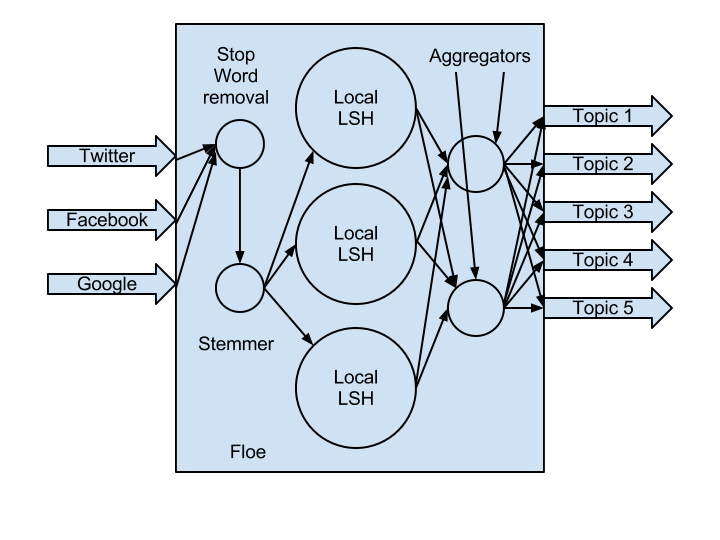
\includegraphics[width=\textwidth]{fig.png}
\end{figure}

There are a number of issues that need to be addressed. First, the hashing functions used over the data items should account for variabilities in same terms used in different messages,  Second, for an unbounded stream, the number of clusters is not bounded and the clustering algorithm should dynamically adjust the parameters and threshold such that desired level of clustering is achieved. Finally, using a single machine to handle the huge and variable data rate may lead to considerable delays in generating the output data streams and the applications consuming these streams that depend on “fresh’’ data will not reflect the up-to-date information. In addition, there may be data burst during a certain period of time, e.g. during Christmas. and the system should be able to handle to handle the fluctuations in the data rate by automatically scaling during such peak periods. 


To address these issues, we propose to extend a distributed Locality Sensitive Hashing [3] and cluster similar topics across different data streams to generate aggregated fresh Topic Streams for Data analysts using FLOE [2], a continuous data flow processing platform that allows custom functions over data streams using a workflow model and allows automatic scaling based on system load. 

\section{Data Sets}
We will mainly be using the data set from Archive.org collected by Calufa. The database consists of 90 million tweets from 6 million users. The sql contains bio data, tweets, link information such as followers and following lists, location, profile name, users. The tweets are time stamped so we can use a stream generator to provide us with a stream. If we do not have data stream from other social networks, we plan to divide this data into multiple parts and generate streams from those data sets. 
We have one more twitter data set collected during a different time but comparatively smaller data set. The data set has also been used in [1]. It consists of tweets and their geographical locations. We can use it as another stream for our purposes.

\section{Major Contribution}
\begin{enumerate}
\item Extend existing LSH algorithm to a distributed environment with online data streams.
\item Develop the online clustering system using a continuous workflow model and demonstrate its feasibility and performance implications.

\end{enumerate}

\section{Milestones}
\begin{enumerate}
\item Month 1: Design distributed LSH for streaming data.
\item Month 2: Implement the online clustering algorithm using Floe.
\item 15 days: Performance analysis and verification of the implementation with real data.
\end{enumerate}


\subsubsection*{References}


\small{

[1] 	Cheng Z., Caverlee J., Lee K., You Are Where You Tweet: A Content-Based Approach to Geo-locating Twitter Users. In Proceeding of the 19th ACM Conference on Information and Knowledge Management (CIKM), Toronto, Oct 2010. \newline
[2] Simmhan Y., Natarajan S., Kumbhare A., Prasanna V., Floe: Designing a Continuous Data Flow Engine for Dynamic Applications on the Cloud, tech report, University of Southern California (submitted). \newline
[3] Wadhwa, S.; Gupta, P.; , "Distributed Locality Sensitivity Hashing," Consumer Communications and Networking Conference (CCNC), 2010 7th IEEE , vol., no., pp.1-4, 9-12 Jan. 2010. \newline
}

\end{document}
